\documentclass{article}
\usepackage{fullpage}
\usepackage{graphicx}
\author{James Gardner}
\date{\today}
\title{NNexus Coding Details}

\begin{document}

\maketitle

{\bf This document outlines the Architecture and Coding Details of NNexus}

\section{Introduction}
This document is written for programmers that are interested in contributing
to the NNexus project and for individuals with programming experience that
would like to aid in bug fixing and reporting. Much of the information in this
introduction section comes from our research paper on NNexus. This section
is optional reading, but may help with understanding what the code is doing
in the NNexus modules. If you wish, you may skip this section and go
directly to the Modules section to get hacking.

Users of NNexus apply the following basic functionality to their corpus:  When an entry is rendered (either at display time or during offline batch processing), the text is broken down into tokens and scanned for words that invoke concepts that have been defined in other entries.  These words (or word tuples) are ultimately turned into hyperlinks to the corresponding entries in the output rendering.

In addition, when new concepts are added to the collection (or the set of concept labels otherwise changes), entries containing potential invocation of these concept labels can be \emph{invalidated}.  This allows entries to be re-scanned for links, either at invalidation time or before the next time they are displayed.
NNexus uses a special structure called the \emph{invalidation index} to facilitate this.

When an article is submitted, NNexus starts by pulling out unlinkable (i.e., equation) environments and other portions of text that need to be escaped.  These portions are replaced by special tokens.  The engine then breaks the text of an entry into a single words/tokens array to iterate through.  This array form makes it easy to associate a particular word with a unique integer position.  

The tokenized text of the entry is then iterated over. The tokens and token tuples (phrases) are then searched to determine candidate links using the concept hash. After the candidate links are determined they are filtered based on linking policies.  The candidates are then compared by ``classification proximity''. The object with the highest score is then the only object left in the match-candidates array. The ``winning'' candidates for each position are then substituted into the original text and the linked document is then returned.


\section{Architecture}
Figure~\ref{arch} contains a high level view of NNexus from a user perspective.
\begin{figure}[ht]
\centerline{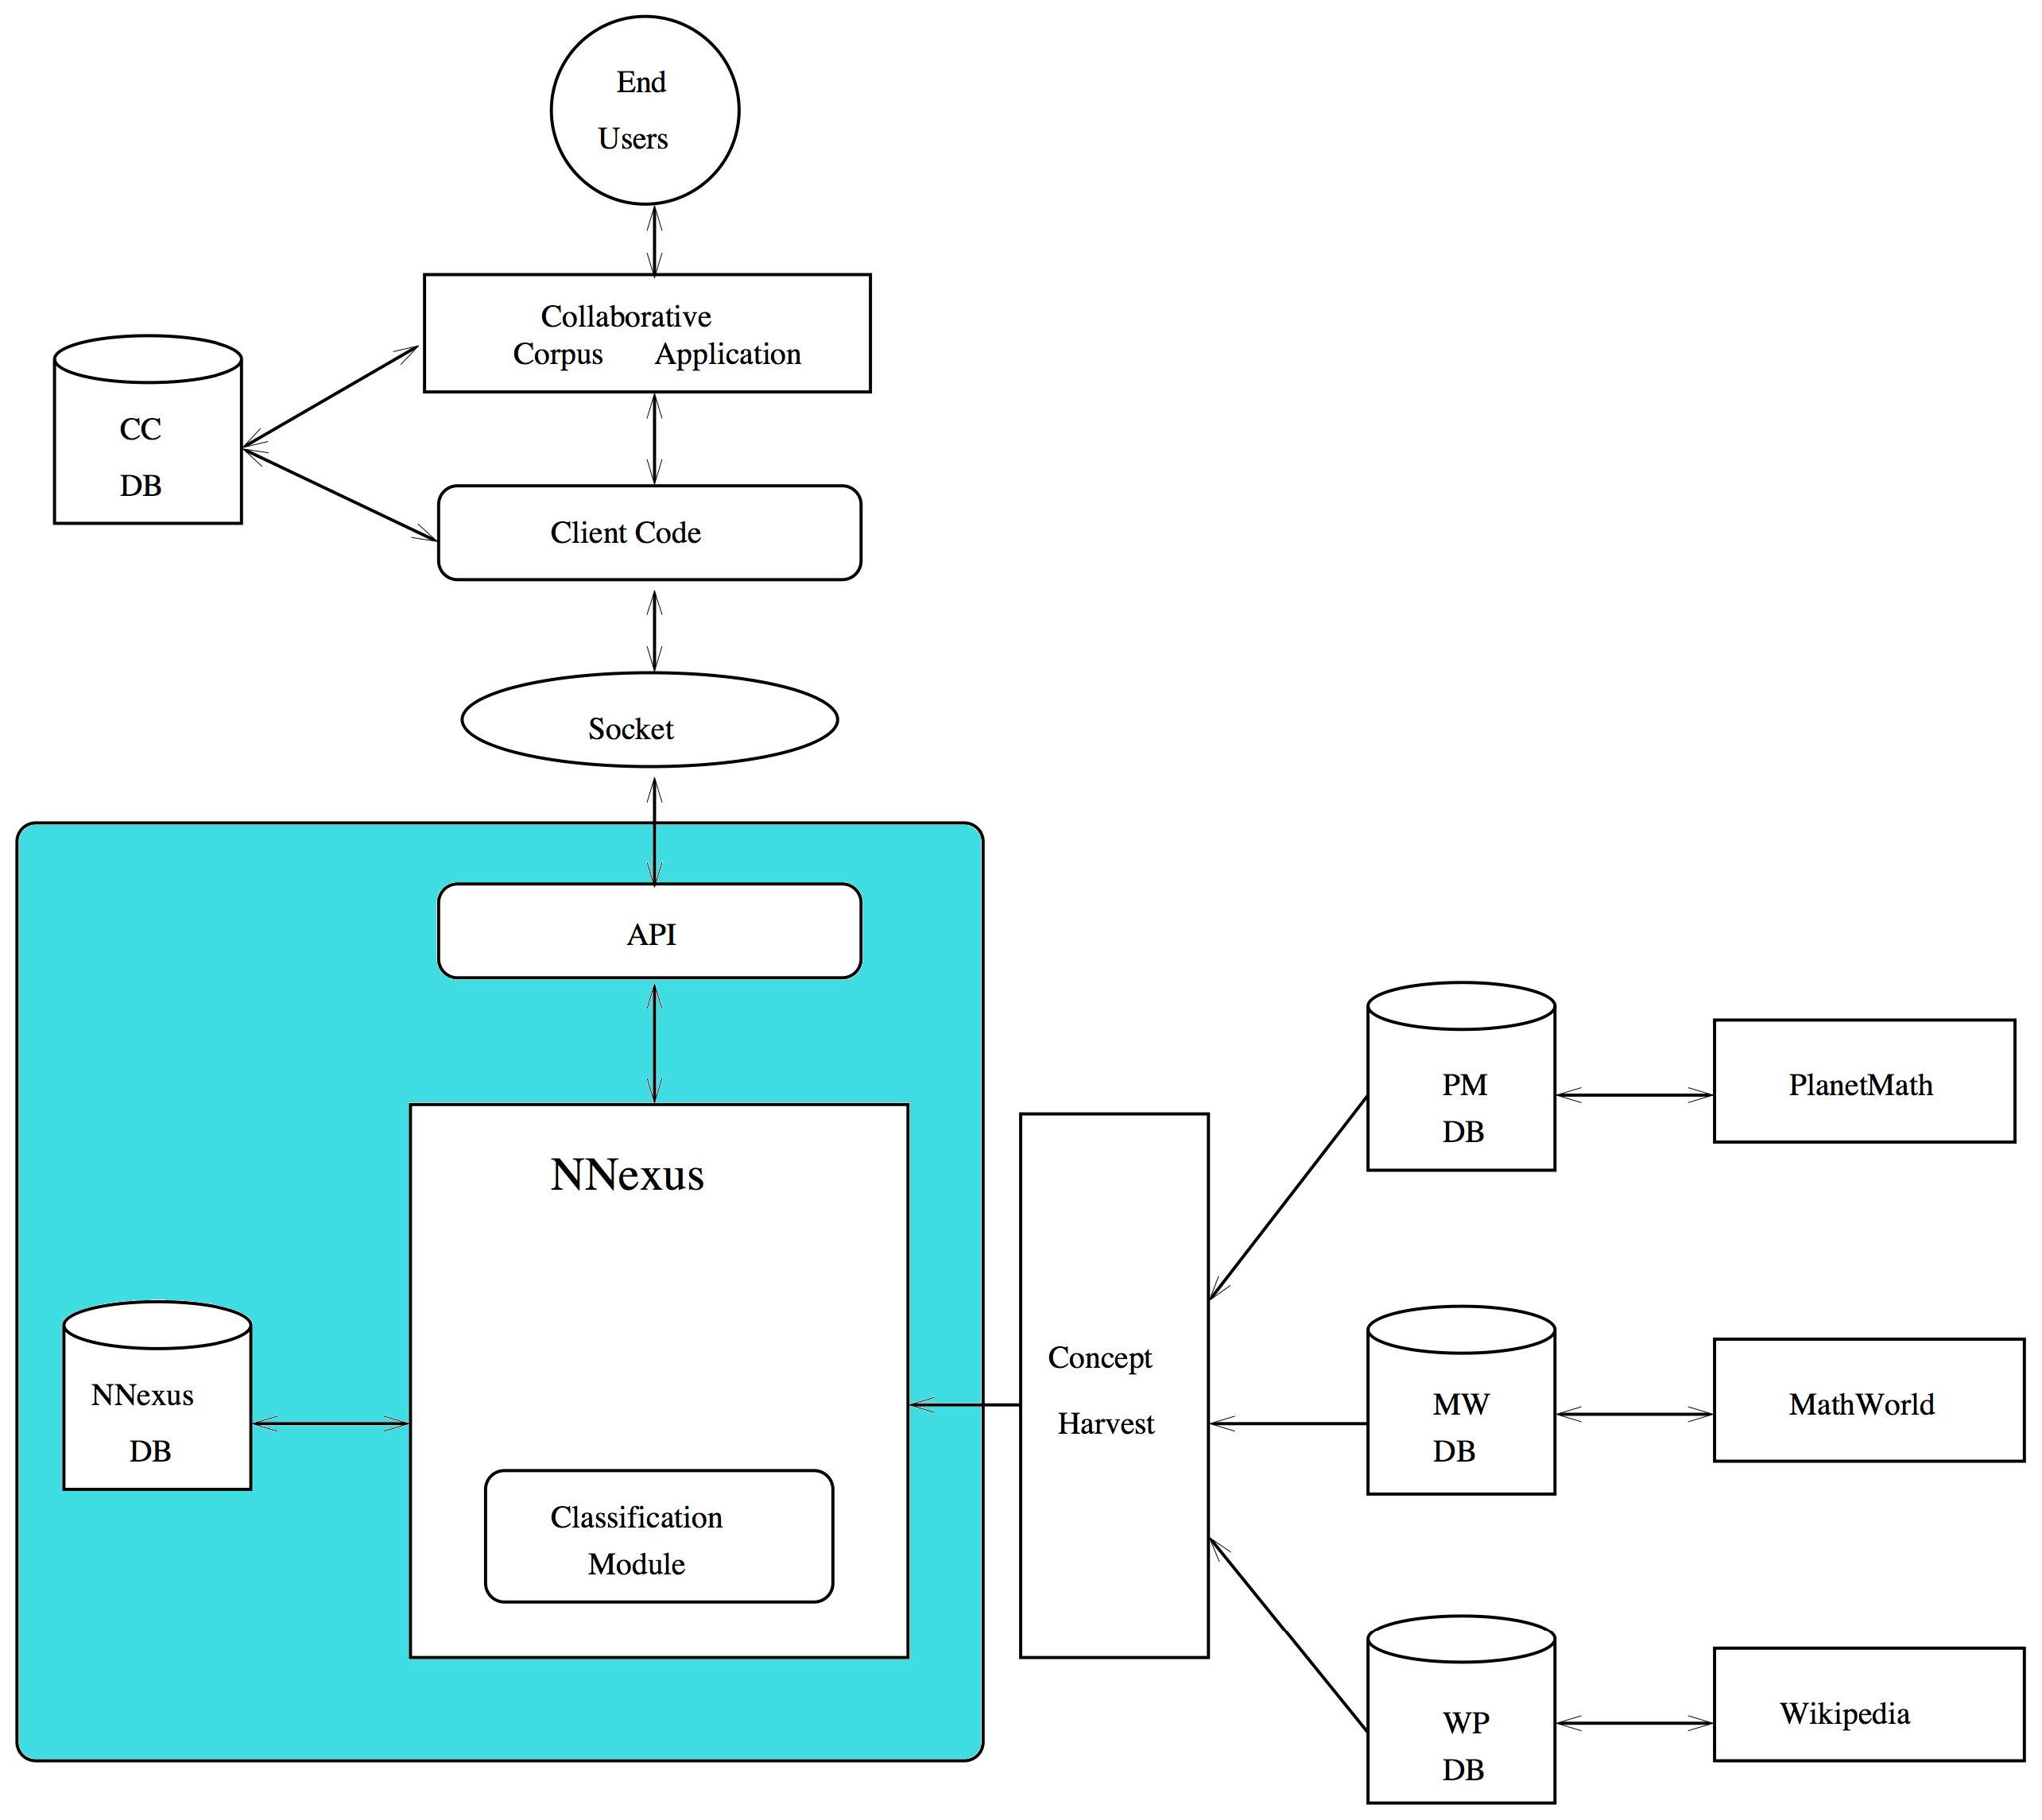
\includegraphics[width=4in]{figures/nnexus-arch}}
\caption{NNexus Architecture}
\label{arch}
\end{figure}


The implementation details follow. NNexus must have a connection to a MySQL
server. The database contains link, object, configuration, and classification
information. The concept map, invalidation index, and classification hierarchy
are all stored in the database.

\subsection{Indexing}
\label{SecIndexing}

NNexus indexes the entries by building a \emph{concept map} that maps all of the concept labels in the corpus to the entries which define these concepts.  The process of building the concept map follows. When adding a new object (entry) to NNexus a list of terms the object defines, synonyms, and a title are provided (the concept labels).

\begin{figure}
\centerline{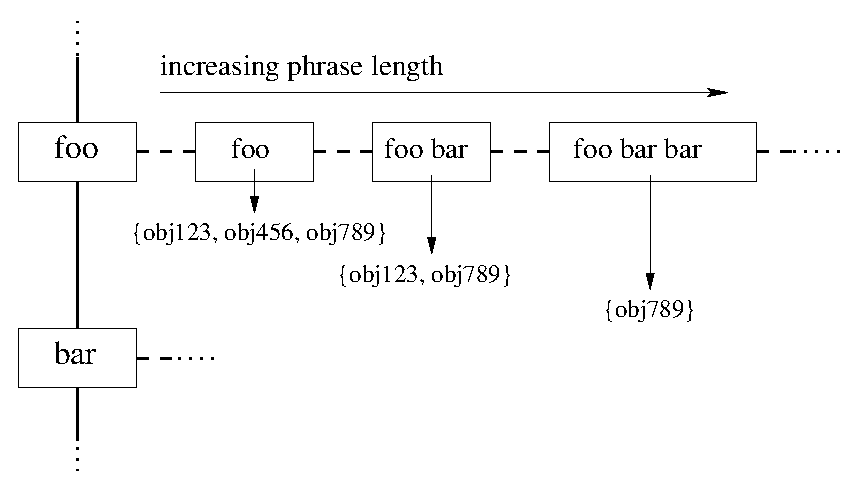
\includegraphics[width=3in]{figures/struct_concept_map}}
\caption{Concept Map: a fast-access (chained-hash-based) structure filled with all the concept labels for all included corpora, used for determining available linking targets as the text is being scanned.}
\label{ConceptMap}
\end{figure}

The concept labels are kept in a chained-hash index structure, called the \emph{concept map}.  This structure contains as keys the words that occur as the first word of some concept label.  Following these words (retrieving the value for the key) leads to a list of full concept labels starting with that particular word. To facilitate efficient scanning of entry text to find concept labels, the map is structured as a chained hash, keyed by the first word of each phrase placed in it. This structure is shown graphically in Figure \ref{ConceptMap}.


When a new object is added, NNexus also utilizes an invalidation index to determine which articles may possibly link to the new object and need to be ``invalidated.'' The invalidation index stores term and phrase \emph{content} information for all entries in the corpus.  It is an adaptive index in that longer phrases are only stored if they appear ``frequently'' in the collection.  There is no limit to how long a stored phrase can be; however, very long phrases are extremely unlikely to appear (the falloff in occurrence count by phrase length follows a Zipf distribution).

\begin{figure}
\centerline{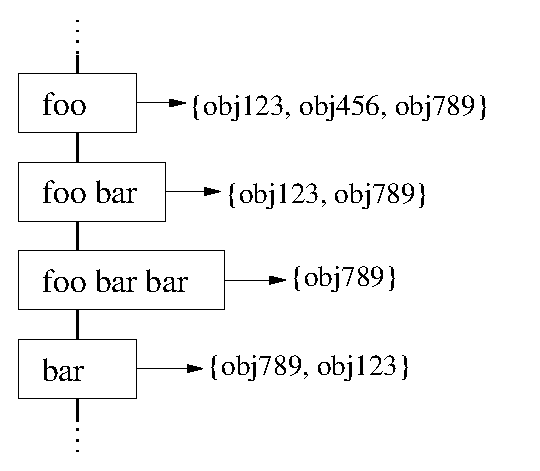
\includegraphics[width=2.6in]{figures/struct_inval}}
\caption{Invalidation Index: an adaptive inverted index containing both words and phrases, used for determining which text objects are likely to need to be re-analyzed for linking after concept definition updates have occurred to the corpus.  The structure is a chained hash, with words and phrases as hash keys, and an object identifier list for each.  In the above example, if a definition for ``foo bar bar'' were added to the corpus, only object 789 would need to be invalidated.}
\label{StructInval}
\end{figure}

The invalidation index is a variation on a normal document inverted index structure and works basically the same way for lookups.  However, instead of just being keyed on single-word terms, it is keyed on phrases (which are usually but not always single-word).   For each term or phrase in the index, there is a list of objects which contain that term or phrase.  These lists are called \emph{postings lists}.  A sketch of the invalidation index is shown in Figure~\ref{StructInval}.

The invalidation index has a special property that for every phrase indexed, all shorter prefixes of that phrase are also indexed for every occurrence of the longer phrase.  This allows us to guarantee that occurrences of the shorter phrases or single terms will be noticed if we do a lookup using these shorter tuples as keys.  The importance of this will be made clear later.

The invalidation index exists for a single purpose: so that when concept labels are added to the collection (or when they change), we can determine which entries are highly likely to be effected by the change.  Further, the invalidation index allows us to do this in a way that never misses an entry that should be re-examined, but does not catch too many irrelevant entries (false positives).

When a lookup is done for a particular phrase in the invalidation index, the object IDs returned are updated (invalidated).


\section{Dependencies}
NNexus was originally developed on Mac OSX with the following software installed:
\begin{itemize}
\item perl-5.8.8 with the following modules installed from CPAN:
\begin{verbatim}
Cwd; DBI; Data::Dumper; Encode; Switch; Time::HiRes;
Unicode::String; XML::SAX; XML::Simple; XML::Writer;
\end{verbatim}
To install any of these modules run \texttt{perl -MCPAN -e shell}. In the shell type \texttt{install Module::Name}. This should install the latest versions of the modules. Note: It is very important to have the latest versions of the XML related modules as all information exchange with NNexus is performed using a strict XML syntax. In order for NNexus to understand all the XML the latest versions of the XML parsers must be installed.

\item
MySQL version 5.0.22 and later are recommended for installation. Note:
NNexus can be run using some older versions of perl and mysql, but this is not guaranteed and may be a headache to get working. We have successfully installed NNexus on a Debian system running Perl version 5.x and MySQL version 4.0, but it wasn't pretty.
\end{itemize}


\section{Modules}
The NNexus system contains the following modules:
\begin{verbatim}
Charset.pm
Classification.pm
Concepts.pm
Config.pm
Crossref.pm
DB.pm
Domain.pm
Indexing.pm
Latex.pm
Linkpolicy.pm
Morphology.pm
NNexusSAXHandler.pm
Object.pm
Response.pm
Util.pm
Utilities.pm
\end{verbatim}

The next few subsections (in alphabetical order for easy reference) cover the details and interactions of these modules.

\subsection{Charset.pm}
The Charset.pm module provides functions that convert between various character
sets and encodings. These functions include converting between international characters and TeX trigraphs (e.g. \"{o} $\rightarrow$ \verb#\"{o}#). These functions are necessary for looking up concepts independent of character set used by the client.

\subsection{Classification.pm}
The Classification.pm module provides functions for accessing, adding, and modifying classification data for objects. Many of the functions included
in this module interact with the MySQL database. This module also contains
functions for determining the similarity of Math Subject Classification (MSC)
categories (e.g. MSC:1024 is more similar to MSC:1022 than MSC:2404.) Note:
This module needs to be updated to support more general classification schemes.
We would like to implement a more general
module that can determine the similarity among categories from multiple
classification schemes. Implementing a new Classification module will allow users from fields other than Mathematics to utilize the automatic linking provided by NNexus.

\subsection{Concepts.pm}
The Concepts.pm module provides function for accessing, adding, and modifying
concept data for objects. Every object in the database defines at least
one concept (if no not explicitly given the concept is the title of the object).
This concept data is stored in a few tables (normal form) on the MySQL server.
Concepts.pm also contains the functions for building the quick lookup concept
hash stored in the database. This module also provides functions for
determining possible linking candidates based on the concepts. More details to come on this section.

\subsection{Config.pm}
The Config.pm module provides functions for accessing the NNexus configuration. It also contains initialization routines for NNexus.

\subsection{Crossref.pm}
The Crossref.pm module is the powerhouse of NNexus. This module contains
the CrossReferenceLaTeX function that accepts an object as input and
outputs the object with links.

Details of almost all of the functions in this module are to come.

\subsection{DB.pm}
The DB.pm modules provides functions for connecting to the MySQL database.

\subsection{Domain.pm}
The Domain.pm module contains functions for accessing domain configuration data, such as priorities and default classification schemes. This module could
conceptually be included in the Config.pm module, but is kept separate for
historic and aesthetic reasons.

\subsection{Indexing.pm}
The Indexing.pm module contains functions for updating the NNexus index
structures in the database. This includes marking objects as valid/invalid
and building the invalidation index. Note: Many of the functions in this module
are old Noosphere code that are no longer called by the NNexus routines.
This module needs be cleaned to indicate that fact that much of the caching routines are specific to Noosphere and have nothing to do with NNexus.

\subsection{Latex.pm}
The Latex.pm module contains functions that parse Latex documents.
This module also determines which Latex tags are visible to the
automatic linker. For example, we don't want sections titles to be linking
so they are not included in the list of visible tags, but we do want
text in \verb#\large# tags to be visible to the automatic linker. We hope this
module becomes either obsolete or greatly reduced soon. The use of regexp
to parse the Latex documents works for now, but a more configurable option
would be to use LaTeX::TOM or another latex parsing method.

\subsection{Linkpolicy.pm}
The Linkpolicy.pm module contains functions that enforce linking policies for
the automatic linker.

\subsection{Morphology.pm}
The Morphology.pm module contains functions that convert between plural, possessive, and mathy phrases. The functions use regular expressions and
a few heuristics to perform these conversions.

\subsection{NNexusSAXHandler.pm}
The NNexusSAXHandler.pm module provides an interface for users to send XML
to NNexus. This XML is then used to determine which internal NNexus routines
should be run and what should be returned.

\subsection{Object.pm}
The Object.pm module provides functions for updating, adding, deleting,
and accessing objects in the NNexus database.

\subsection{Response.pm}
The Response.pm module handles responses to client request. The functions
in this module build XML documents to return back to the clients.

\subsection{Util.pm}
The Util.pm module provides utility functions for manipulating and modifying
html documents and files. These functions are kept historically from the Noosphere project.

\section{Module Interaction}
The module dependency graph is shown in Figure~\ref{Modules}
\begin{figure}[ht]
\centerline{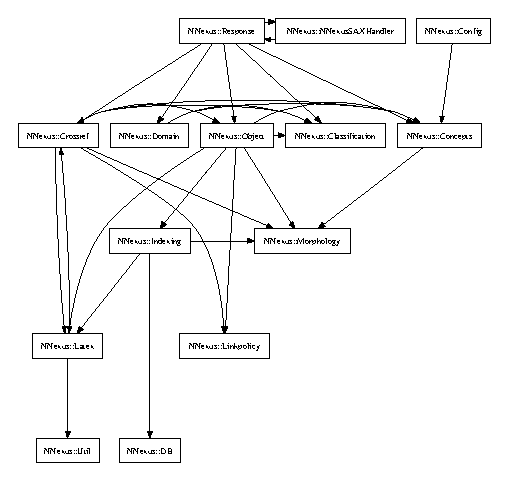
\includegraphics[width=5.5in]{figures/NNexusModuleDep}}
\caption{Module Dependencies for NNexus System}
\label{Modules}
\end{figure}


\end{document}
